\section{Assistentes virtuais}

Assistentes virtuais são sistemas computacionais projetados para interagir com seres humanos de forma natural, simulando comunicação e execução de tarefas via interfaces digitais \cite{cruz_assistentes_2018}. Seu objetivo principal é facilitar o acesso à informação, automatizar processos, responder perguntas, realizar comandos e oferecer suporte personalizado em diversos contextos, desde o atendimento ao cliente até a automação residencial e corporativa. A \autoref{fig:funcionamento-assistente} esquematiza o funcionamento simplificado de um assistente virtual.


\begin{figure}[H]
    \caption{Funcionamento simplificado de um assistente virtual.}
    \label{fig:funcionamento-assistente}
    \centering
    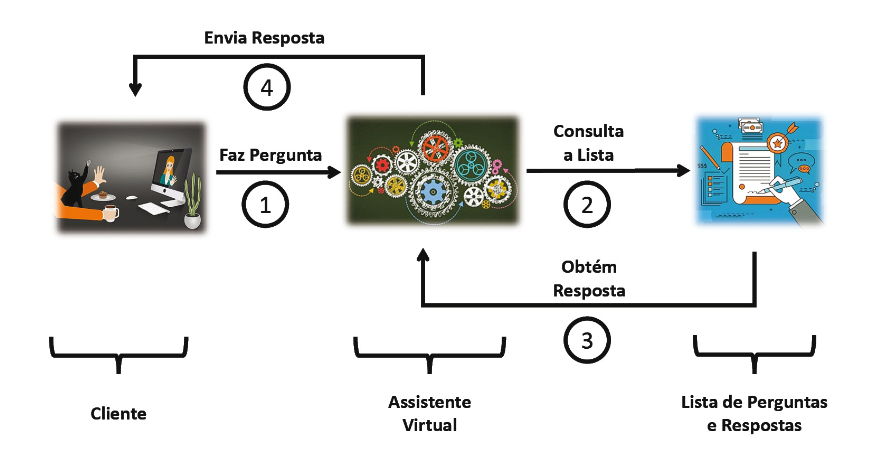
\includegraphics[width=\linewidth, height=8cm]{imagens/2-funcionamento-assistente-virtual.png}    
    {\par \raggedright \footnotesize Fonte: \textcite{cruz_assistentes_2018}.\par}
\end{figure}



A arquitetura de um assistente virtual é composta por diferentes módulos especializados, que trabalham de forma integrada para compreender, processar e responder às solicitações dos usuários. Os principais componentes incluem:

\begin{itemize}
  \item \textbf{Reconhecimento de fala (Speech-to-Text)}: Converte comandos de voz em texto, permitindo que o assistente compreenda solicitações verbais.
    \item \textbf{Processamento de linguagem natural (Text-to-Text)}: Interpreta o texto recebido, identifica intenções, extrai entidades e gera respostas adequadas.
    \item \textbf{Síntese de fala (Text-to-Speech)}: Transforma textos em áudio, possibilitando respostas em voz natural.
    \item \textbf{Módulos de integração}: Conectam o assistente a sistemas externos, bancos de dados, \gls{api}s e dispositivos inteligentes.
    \item \textbf{Gestão de contexto}: Mantém o histórico de interações, permitindo diálogos contínuos e personalizados.
\end{itemize}

Os assistentes virtuais são impulsionados por um conjunto de tecnologias de \acrfull{ia}, nas quais sistemas de \gls{ml} e \gls{dl} possibilitam o reconhecimento de padrões em voz e linguagem, bem como a personalização de interações, enquanto a própria \gls{ia} viabiliza a compreensão semântica e a tomada de decisão. Um marco revolucionário nessa área foi a introdução da arquitetura Transformer em 2017 \cite{vaswani_attention_2017}, que transformou o \gls{nlp} por meio de mecanismos de atenção — base dos atuais \gls{llm}, como ChatGPT e Gemini, conforme ilustrado na \autoref{fig:transformers}. A integração desses \gls{llm} generativos elevou substancialmente a capacidade de processamento de linguagem natural, permitindo a interpretação de nuances, a geração criativa de respostas e a adaptação contextual do tom comunicativo. Como resultado, ampliaram-se significativamente as aplicações práticas desses sistemas, que passaram a abranger desde atendimento automatizado e suporte técnico até a criação de conteúdo estruturado e a análise de dados complexos \cite{mckinsey_economic_2023}.

Nesse contexto, os assistentes virtuais consolidam-se como ferramentas interativas inovadoras, que utilizam \gls{nlp} e \gls{ia} para estabelecer comunicação direta e intuitiva com os usuários. Por meio de comandos de voz ou texto, tais sistemas respondem a perguntas, executam operações financeiras e oferecem orientações personalizadas — cobrindo desde demandas cotidianas até tarefas de maior complexidade, como recomendações de investimentos e simulações de crédito \cite{cruz_assistentes_2018}.

\begin{figure}[H]
    \caption{Evolução dos modelos de conversação.}
    \label{fig:transformers}
    \centering
    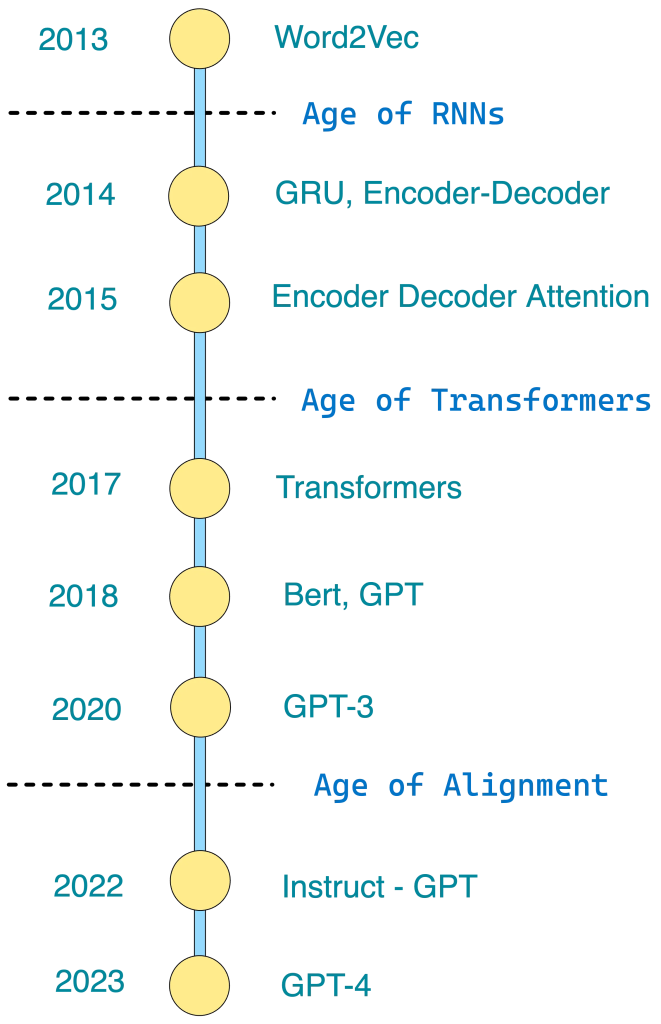
\includegraphics[width=0.3\linewidth]{imagens/4-transformers.png}    
    {\par \raggedright \footnotesize Fonte: \textcite{dsacademy_llms_2023}.\par}
\end{figure}

Apesar dos avanços, a adoção de grandes modelos de \gls{ia} generativa apresenta desafios significativos relacionados ao consumo intensivo de recursos computacionais e ao impacto na latência do sistema. Estudos acadêmicos demonstram que o treinamento de modelos como o GPT-3 demanda aproximadamente 1.287 megawatt-horas (MWh), equivalente ao consumo anual médio de 420 pessoas \cite{argerich_measuring_2024}. Durante a inferência, pesquisas mostram que modelos como o Bloom consomem aproximadamente 3,96 watt-horas por requisição \cite{argerich_measuring_2024}, enquanto aplicações como ChatGPT podem demandar mais de 1.500 MWh mensalmente considerando 13 milhões de usuários diários. A latência e o tempo de resposta são diretamente afetados pela complexidade dos modelos, onde a relação entre número de parâmetros e operações computacionais (aproximadamente duas vezes o número de parâmetros por token gerado) impacta significativamente o desempenho \cite{argerich_measuring_2024}, podendo comprometer a experiência do usuário em aplicações que requerem respostas em tempo real, especialmente no setor financeiro onde a rapidez de processamento é crítica para operações sensíveis ao tempo.


\subsection{Aplicações de Assistentes Virtuais baseadas em microsserviços no setor financeiro}

Nos últimos anos, o setor financeiro tem desenvolvido soluções tecnológicas sofisticadas que integram assistentes virtuais a complexos bancos de dados e arquiteturas distribuídas. Essas implementações incluem plataformas de análise preditiva para avaliação de crédito e detecção de fraudes, sistemas de automação de \textit{back-office}, e soluções de personalização que utilizam \gls{llm} e \gls{ia} Multimodal para enriquecer a análise de dados financeiros \cite{febraban_estudo_2024}. O investimento massivo nessas tecnologias reflete a busca por maior eficiência operacional e redução de custos, com a tecnologia sendo vista como um grande diferencial competitivo entre as instituições bancárias.

Essa convergência entre assistentes virtuais inteligentes e arquiteturas de microsserviços redefine a prestação de serviços financeiros, criando um ecossistema tecnológico ágil, escalável e eficiente. Estudos recentes da Febraban em colaboração com a Accenture demonstram que a \gls{ia} Generativa pode aumentar a eficiência dos bancos entre 25\% e 35\% \cite{febraban_estudo_2024}, enquanto pesquisa da IBM indica que a adoção estratégica dessa tecnologia pode elevar significativamente o desempenho financeiro das instituições \cite{ibm_2025_2025}. Esta transformação é particularmente relevante em um contexto onde microsserviços permitem desenvolvimento, otimização e dimensionamento independente de cada etapa do processamento de \gls{ia}, desde o pré-processamento de dados até a inferência de modelo e pós-processamento \cite{nvidia_decodificando_2024}.

No Brasil, exemplos práticos demonstram a maturidade dessa abordagem arquitetural. A \textbf{Bia (Bradesco Inteligência Artificial)} atende 3 milhões de clientes como assistente virtual multimodal, processando milhões de interações mensais sobre produtos financeiros através de múltiplos canais \cite{valor_investe_os_2025}. O \textbf{Banco do Brasil} desenvolveu a ferramenta "Ari" (Área de Recomendações Inteligentes), que já gerou mais de 60 milhões de recomendações personalizadas, impactando 2,5 milhões de micro e pequenos empresários com insights sobre volume de vendas, produtos financeiros e detecção de inadimplência \cite{valor_investe_os_2025}. Paralelamente, \textit{fintechs} como a \textbf{Magnetis} utilizam arquiteturas distribuídas para oferecer consultoria de investimentos automatizada, enquanto a \textbf{Accountfy} implementou assistentes virtuais com \gls{ia} integrados em sua plataforma SaaS para otimizar a governança financeira empresarial \cite{accountfy_assistentes_2024}.

A capacidade desses assistentes de interpretar e executar comandos em tempo real os torna ideais para bancos e \textit{fintechs} que buscam atendimento de alta qualidade e redução de custos operacionais. A arquitetura de microsserviços, comumente aplicada, permite que os assistentes integrem múltiplos módulos de dados de forma independente e escalável, aumentando a eficiência e facilitando a personalização de serviços \cite{villamizar_evaluating_2023}. A Interface desses sistemas se foca na interação por voz, visando uma comunicação mais natural e eficiente entre usuário e sistema, acompanhando o advento de ambientes tecnológicos cada vez mais conectados e sofisticados.